% D.4.3 Project Full Application Report -- Overleaf / IEEEtran source
% Before submission: replace the author details and project-management link below.
\documentclass[conference]{IEEEtran}
\usepackage{graphicx}
\usepackage{booktabs}
\usepackage{array}
\usepackage{url}
\usepackage{hyperref}
\usepackage{listings}
\usepackage{xcolor}
\usepackage{tikz}
\usetikzlibrary{positioning,arrows.meta,shapes.geometric}
\hypersetup{colorlinks=true,urlcolor=blue,citecolor=blue,linkcolor=blue}
\definecolor{codegray}{RGB}{245,245,245}
\lstset{basicstyle=\ttfamily\footnotesize,backgroundcolor=\color{codegray},frame=single,breaklines=true}
\newcommand{\repo}{\url{https://github.com/pruthvi4344/bug-deduplication-pgvector}}
% REQUIRED: Replace the values in this block before submission.
\newcommand{\pmtool}{\textit{[Insert accessible Jira/Hive/Trello project-management link]}}
\newcommand{\memberone}{\textit{[Member 1 name, student ID, UWindsor email]}}
\newcommand{\membertwo}{\textit{[Member 2 name, student ID, UWindsor email]}}
\newcommand{\memberthree}{\textit{[Member 3 name, student ID, UWindsor email]}}
\newcommand{\memberfour}{\textit{[Member 4 name, student ID, UWindsor email]}}

\begin{document}
\title{AI Bug Deduplication System using PostgreSQL pgvector}
\author{\IEEEauthorblockN{\memberone \and \membertwo \and \memberthree \and \memberfour}
\IEEEauthorblockA{Master of Applied Computing\\University of Windsor, Windsor, Canada}}
\maketitle

\begin{abstract}
Software projects frequently receive multiple bug reports that describe the same underlying defect using different wording. Manual duplicate triage is slow, inconsistent, and costly. This project implements an AI Bug Deduplication System that converts Bugzilla-style reports into semantic vectors using the \texttt{sentence-transformers/all-MiniLM-L6-v2} model, stores 384-dimensional embeddings in PostgreSQL through pgvector, and retrieves likely duplicates with cosine-similarity search. The application provides a React dashboard, a FastAPI backend, CSV import, hybrid metadata filtering, exact vector search, and two approximate nearest-neighbour (ANN) index methods: HNSW and IVFFlat. A benchmark module compares ANN output with an exact PostgreSQL cosine-similarity baseline and persists Recall@1, Recall@5, Recall@10, average latency, and p95 latency. The delivered application was verified on 103 reports with 384-dimensional embeddings; an HNSW benchmark over 20 sampled queries achieved 100\% Recall@1, Recall@5, and Recall@10 with 13.68 ms average latency and 17.70 ms p95 latency. This report documents the architecture, source files, data, database schema, project-management process, and reproducible local deployment required for D.4.3.
\end{abstract}
\begin{IEEEkeywords}
bug deduplication, semantic search, PostgreSQL, pgvector, HNSW, IVFFlat, Sentence-BERT, cosine similarity
\end{IEEEkeywords}

\section{Introduction}
Bug trackers accumulate duplicate reports because different reporters describe the same fault with different vocabulary, environments, and levels of detail. Lexical matching alone may fail to identify that ``preferences dialog causes an immediate exit'' and ``browser crashes when opening settings'' describe the same defect. The AI Bug Deduplication System supports human triage by ranking historical reports according to semantic similarity. It does not automatically close or modify reports; a triager remains responsible for the final duplicate decision.

The application cleans source text, generates embeddings with \texttt{all-MiniLM-L6-v2}, persists the result in PostgreSQL 16 with pgvector, and performs top-$k$ cosine retrieval in the same database that holds the relational bug metadata. Product and component values can be used as hybrid filters. The implementation supports exact, HNSW, and IVFFlat modes so quality and response-time trade-offs can be evaluated rather than assumed.

\section{System Architecture}
Fig.~\ref{fig:architecture} shows the high-level design. The browser-facing React/Vite dashboard provides import, search, benchmark, and information views. FastAPI validates requests through Pydantic schemas and coordinates cleaning, embedding, search, and benchmark services. PostgreSQL plus pgvector stores both relational fields and vectors. HNSW and IVFFlat provide ANN access methods, while exact cosine retrieval serves as the benchmark ground truth.

\begin{figure*}[!t]
\centering
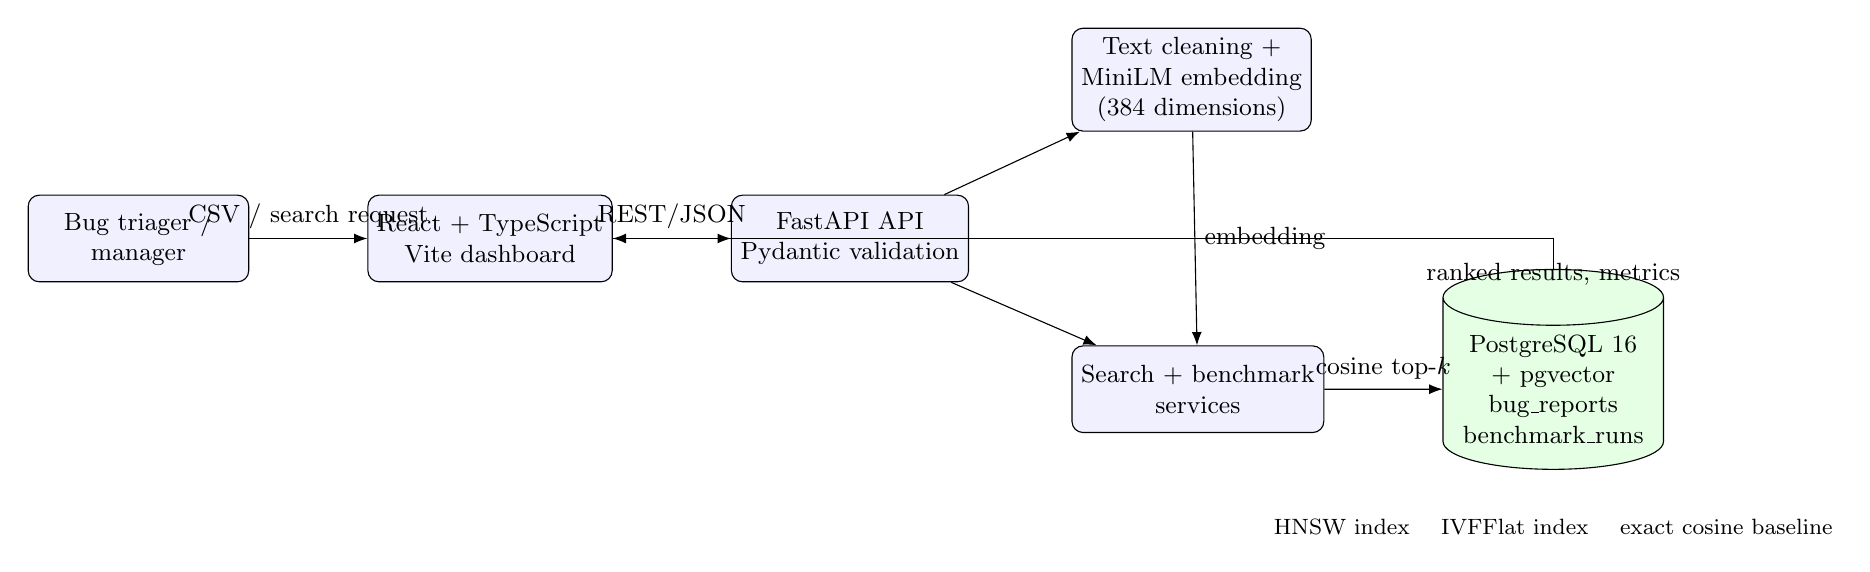
\begin{tikzpicture}[node distance=11mm and 15mm, >=Latex, every node/.style={font=\small}, box/.style={draw, rounded corners, align=center, minimum width=28mm, minimum height=11mm, fill=blue!6}, db/.style={draw, cylinder, shape border rotate=90, aspect=.28, align=center, minimum width=28mm, minimum height=18mm, fill=green!10}]
\node[box] (user) {Bug triager /\\manager};
\node[box, right=of user] (web) {React + TypeScript\\Vite dashboard};
\node[box, right=of web] (api) {FastAPI API\\Pydantic validation};
\node[box, above right=8mm and 13mm of api] (ai) {Text cleaning +\\MiniLM embedding\\(384 dimensions)};
\node[box, below right=8mm and 13mm of api] (service) {Search + benchmark\\services};
\node[db, right=of service] (db) {PostgreSQL 16\\+ pgvector\\\small bug\_reports\\benchmark\_runs};
\draw[->] (user) -- node[above]{CSV / search request} (web);
\draw[->] (web) -- node[above]{REST/JSON} (api);
\draw[->] (api) -- (ai);
\draw[->] (ai) -- node[right]{embedding} (service);
\draw[->] (api) -- (service);
\draw[->] (service) -- node[above]{cosine top-$k$} (db);
\draw[->] (db) |- node[pos=.25,below]{ranked results, metrics} (web);
\node[below=5mm of db, align=center, font=\footnotesize] {HNSW index \quad IVFFlat index \quad exact cosine baseline};
\end{tikzpicture}
\caption{Logical architecture of the AI Bug Deduplication System.}
\label{fig:architecture}
\end{figure*}

\subsection{Embedding and Retrieval Pipeline}
For each report, the system combines the summary and description, decodes HTML entities, removes HTML tags and URLs, and normalizes whitespace. The cleaned text is encoded by MiniLM into a unit-normalized vector containing 384 floating-point values. A user query follows the identical pipeline, ensuring that documents and queries occupy the same embedding space. PostgreSQL computes vector distance with pgvector cosine operators; similarity displayed in the user interface is $1 - \mathrm{cosine\ distance}$.

\subsection{ANN and Exact Modes}
HNSW uses a navigable graph with $m=16$ and \texttt{ef\_construction=64}. At search time, the application sets \texttt{hnsw.ef\_search=80}. IVFFlat partitions the vector space into lists and uses \texttt{ivfflat.probes=20}; for the 103-report local dataset, the index was rebuilt with 10 lists after data import. Exact mode disables index and bitmap scans for its baseline transaction, preventing ANN retrieval from contaminating Recall@K calculations.

\section{Source Code Organization}
The repository is a full-stack project. Table~\ref{tab:source} lists the primary files and responsibilities. The source uses Python type annotations, docstrings, structured Pydantic models, and explanatory inline comments. The GitHub repository is the authoritative, current location of all source code, executable definitions, database scripts, data files, documentation, and configuration examples.

\begin{table*}[!t]
\caption{Primary source files and responsibilities}
\label{tab:source}
\centering
\begin{tabular}{p{.28\textwidth}p{.64\textwidth}}
\toprule
\textbf{File or directory} & \textbf{Responsibility}\\
\midrule
\texttt{backend/app/main.py} & FastAPI application, health endpoint, CSV-import endpoint, search endpoint, benchmark endpoints, CORS configuration, and API error translation.\\
\texttt{backend/app/services.py} & Text cleaning, cached MiniLM model loading, embedding creation, hybrid vector retrieval, and Recall@K/latency benchmarking.\\
\texttt{backend/app/models.py} & SQLAlchemy models for \texttt{bug\_reports} and \texttt{benchmark\_runs}; pgvector \texttt{Vector(384)} mapping.\\
\texttt{backend/app/schemas.py} & Pydantic request/response schemas and validation constraints.\\
\texttt{backend/app/database.py}, \texttt{config.py} & Database session lifecycle and environment-driven configuration.\\
\texttt{frontend/src/App.tsx} & React pages for Home/import, duplicate Search, Benchmarks, and About.\\
\texttt{frontend/src/api.ts} & Typed client calls to the FastAPI endpoints.\\
\texttt{frontend/src/components/ui.tsx} & Navigation, similarity badge, and loading-spinner components.\\
\texttt{database/production\_schema.sql} & pgvector extension, relational schema, validation constraints, and update trigger.\\
\texttt{database/production\_indexes.sql} & B-tree hybrid-filter indexes plus HNSW and IVFFlat vector indexes.\\
\texttt{docker-compose.yml} & Reproducible PostgreSQL/pgvector, API, and web-service deployment.\\
\texttt{requirements.txt}, \texttt{frontend/package.json} & Python and JavaScript dependency manifests.\\
\bottomrule
\end{tabular}
\end{table*}

Listing~\ref{lst:search} is a representative implementation excerpt. It demonstrates that metadata filtering and cosine vector ranking are composed in one SQLAlchemy query path.
\begin{lstlisting}[caption={Hybrid vector-retrieval excerpt from \texttt{services.py}.},label={lst:search},language=Python]
distance = BugReport.embedding.cosine_distance(embed(request.query))
stmt = select(BugReport, (1 - distance).label("similarity"))
if request.product:
    stmt = stmt.where(BugReport.product == request.product)
if request.component:
    stmt = stmt.where(BugReport.component == request.component)
if request.exclude_id:
    stmt = stmt.where(BugReport.id != request.exclude_id)
return db.execute(stmt.order_by(distance).limit(request.k)).all()
\end{lstlisting}

\section{Executables and Auxiliary Files}
The application does not ship platform-specific binary executables. Its runnable artifacts are Docker images built from \texttt{backend/Dockerfile} and \texttt{frontend/Dockerfile}; Docker Compose is the primary executable/deployment interface. The API image runs Uvicorn with \texttt{backend.app.main:app}; the web image builds the Vite client and serves it through NGINX. Supporting materials include the environment example, database initialization scripts, raw and processed data folders, tests, project documentation, and README instructions.

The primary command for a complete build and launch is:
\begin{lstlisting}[language=bash]
docker compose up --build
\end{lstlisting}
The dashboard is then available at \url{http://localhost:5173}, the health endpoint at \url{http://localhost:8000/health}, and interactive OpenAPI documentation at \url{http://localhost:8000/docs}.

\section{Dataset}
The project includes a small Bugzilla-format seed dataset and a larger local test dataset named \texttt{mozilla\_firefox\_100.csv}. The latter contains 100 public Firefox reports obtained from Mozilla's public Bugzilla REST API. Together with the three seed records, the verified local deployment contains 103 reports. Each row has a Bugzilla identifier, summary, description field, product/component metadata where available, resolution status, operating system, architecture, and an embedding generated at import time.

The CSV importer accepts \texttt{bug\_id}, \texttt{summary}, \texttt{description}, \texttt{product}, \texttt{component}, \texttt{resolution\_status}, \texttt{operating\_system}, and \texttt{architecture}. The report data is public Bugzilla metadata; its source API and collection method are documented in the repository README and deployment documentation. The data source is Mozilla Bugzilla \cite{mozillaapi}.

\begin{table}[!t]
\caption{Verified local dataset state}
\label{tab:data}
\centering
\begin{tabular}{ll}
\toprule
\textbf{Item} & \textbf{Value}\\
\midrule
Seed reports & 3\\
Mozilla Firefox reports & 100\\
Total stored reports & 103\\
Embedding model & all-MiniLM-L6-v2\\
Embedding dimension & 384\\
Similarity metric & cosine similarity\\
\bottomrule
\end{tabular}
\end{table}

\section{Database Schema and Connection Instructions}
PostgreSQL 16 with the pgvector extension is the project database. The \texttt{bug\_reports} table stores the report source fields and a required \texttt{vector(384)} embedding. \texttt{external\_id} is unique when populated, so re-importing an identical Bugzilla CSV is rejected safely. \texttt{benchmark\_runs} stores the selected index type, $k$, evaluated query count, Recall@1/@5/@10, average latency, p95 latency, and timestamp.

The system was verified using three relevant indexes: \texttt{idx\_bug\_hnsw} with cosine operations, \texttt{idx\_bug\_ivfflat} with cosine operations, and a composite B-tree index on \texttt{(product, component)} for hybrid filtering. A status B-tree index also supports status-based relational queries. All 103 stored embeddings were validated with \texttt{vector\_dims(embedding) = 384}.

\subsection{Local Connection and Run Procedure}
The database runs inside the Compose-managed \texttt{db} service. A grader needs Docker Desktop; a separate native PostgreSQL installation is not required. From the cloned repository root, run:
\begin{lstlisting}[language=bash]
docker compose up --build
\end{lstlisting}
PostgreSQL is internally available to the API as \texttt{postgresql+psycopg://postgres:postgres@db:5432/bugdedup}. The host mapping is port 5432. To inspect the database locally:
\begin{lstlisting}[language=bash]
docker compose exec db psql -U postgres -d bugdedup
\end{lstlisting}
The first start initializes the vector extension, schema, trigger, and indexes through the SQL scripts mounted in \texttt{docker-entrypoint-initdb.d}. After bulk import, IVFFlat should be rebuilt with a list count appropriate to the collection size; the verified 103-row installation used \texttt{lists=10}.

\section{Deployment and Access for Grading}
The project is deployed as a local Docker Compose application, not on a cloud-hosted public server. This is stated explicitly because the application requires PostgreSQL with pgvector and SentenceTransformer model loading. The public GitHub repository is the main project portal and is accessible to graders at \repo. It contains source code, Docker configuration, schema/index scripts, sample data, README, and D.4 documentation.

A grader can run the application without separately installing Python, Node.js, PostgreSQL, or pgvector: install Docker Desktop, clone the repository, run \texttt{docker compose up --build}, then open the local dashboard. The first model use may download the MiniLM model, after which imported reports can be searched and benchmarked. This local, containerized approach is the personal platform used to host the working application for assessment.

\section{Evaluation}
The dashboard's benchmark module measures approximate results against exact PostgreSQL cosine search. For each sampled report, it retrieves ANN candidates, executes an exact baseline query, records whether the result sets overlap at $k=1$, $5$, and $10, and persists response time. The verified HNSW run sampled 20 reports from the 103-report collection and obtained the results in Table~\ref{tab:benchmark}.

\begin{table}[!t]
\caption{Verified HNSW benchmark result}
\label{tab:benchmark}
\centering
\begin{tabular}{ll}
\toprule
\textbf{Metric} & \textbf{Observed result}\\
\midrule
Index type & HNSW\\
Queries evaluated & 20\\
Recall@1 & 100.0\%\\
Recall@5 & 100.0\%\\
Recall@10 & 100.0\%\\
Average latency & 13.68 ms\\
P95 latency & 17.70 ms\\
\bottomrule
\end{tabular}
\end{table}

These values demonstrate correct end-to-end functionality on the local dataset. They must not be generalized as a claim of universal 100\% recall at production-scale data volumes; a larger corpus and repeated experiments are necessary for a final performance conclusion. IVFFlat and exact modes were also tested through the OpenAPI interface on the same query and returned the same leading duplicate candidates as the HNSW dashboard search.

\section{Project Management Principles}
The team used a separate project-management workspace to plan, assign, track, and review tasks. The accessible project-management link must be placed in Section~\ref{sec:links} before submission. The codebase follows modular decomposition: the backend persistence/API layer, embedding/search/benchmark service layer, frontend dashboard layer, and database deployment layer have clear boundaries. This structure supports parallel development, isolated testing, and lower merge-conflict risk.

The project also followed iterative validation. First, the Docker stack was launched and health/API documentation endpoints were verified. Next, seed reports were imported and searched. Then 100 public Firefox Bugzilla records were imported, all 103 384-dimensional embeddings were verified, HNSW and IVFFlat indexes were confirmed in PostgreSQL, and benchmark results were recorded. This sequence creates traceable evidence that each subsystem functions before full integration claims are made.

\section{Repository and Project Management Links}\label{sec:links}
\begin{itemize}
\item \textbf{Code repository and main project portal:} \repo
\item \textbf{Project-management tool:} \pmtool
\item \textbf{Application hosting platform:} Local Docker Compose deployment; setup command: \texttt{docker compose up --build}. No cloud-hosted URL is claimed.
\end{itemize}

\section{Conclusion}
The AI Bug Deduplication System demonstrates a complete database-centered semantic search workflow. It imports Bugzilla-style reports, generates 384-dimensional sentence embeddings, stores them in PostgreSQL pgvector, retrieves similar reports using cosine similarity, and exposes HNSW, IVFFlat, and exact modes for evaluation. The delivered Docker Compose project, public repository, source code, dataset assets, database schema, and run instructions provide a reproducible D.4.3 submission. The verified local deployment demonstrates correct vector storage, duplicate retrieval, ANN indexing, and benchmark persistence while retaining the human triager as the final decision maker.

\begin{thebibliography}{1}
\bibitem{mozillaapi} Mozilla, ``Bugzilla REST API,'' Mozilla Bugzilla. [Online]. Available: \url{https://bugzilla.mozilla.org/rest/bug}. Accessed: Aug. 3, 2026.
\bibitem{pgvector} pgvector contributors, ``pgvector: Open-source vector similarity search for Postgres.'' [Online]. Available: \url{https://github.com/pgvector/pgvector}.
\bibitem{minilm} N. Reimers and I. Gurevych, ``Sentence-BERT: Sentence Embeddings using Siamese BERT-Networks,'' in \textit{Proc. EMNLP}, 2019.
\end{thebibliography}
\end{document}
